\documentclass{article}
\usepackage[utf8]{inputenc}
\usepackage{hyperref}
\usepackage{geometry}
%Mettere le foto sulla stessa
\usepackage{subcaption}
%lib img
\usepackage{natbib}
\usepackage{graphicx}
\hypersetup{
    colorlinks=true,
    linkcolor=red,
    filecolor=red,      
    urlcolor=red,
}
%impaginazione margini ecc...
\geometry{a4paper, top=3cm, bottom=3cm, left=2.5 cm, right=3.5cm }
\title{Script}
\author{a.daguanno1 }
\date{April 2021}

\begin{document}

\maketitle

\section{Introduction}
\section{Compiler}
\begin{itemize}
    \item\url{https://www.python.org/downloads/release/python-394/}
\end{itemize}
\section{Library Script}
\subsection{Anaconda}
Anaconda è una distribuzione dei linguaggi di programmazione Python per il calcolo scientifico. Che mira a semplificare la gestione e la distribuzione dei pacchetti.
\\Racchiude in se il compilatore python, un pakage enviroment "Conda" che ci consente di istallare i package 
\begin{itemize}
    \item\url{https://www.anaconda.com/products/individual/download-success}
    \item\url{https://www.youtube.com/watch?v=UmORrAvr4pQ}
\end{itemize}
\begin{enumerate}
    \item Avviamo l'istallazione
    \item Avviamo poi Anaconda Navigator l'app istallata
    \item Cerchiamo una libreria andado sulla sinistra nella voce "Environments" e cercando ad es "numpy"
\end{enumerate}

\textbf{Creare il proprio environment}
\begin{enumerate}
    \item In Environmets in Anacoda Navigator cliccare si create in basso a sinistra 
    \item Inserire un titolo
    \item Cercare poi i package che si devono utilizzare nell'ambiente del progetto ed installarli 
    \begin{figure}[h!]
        \centering
        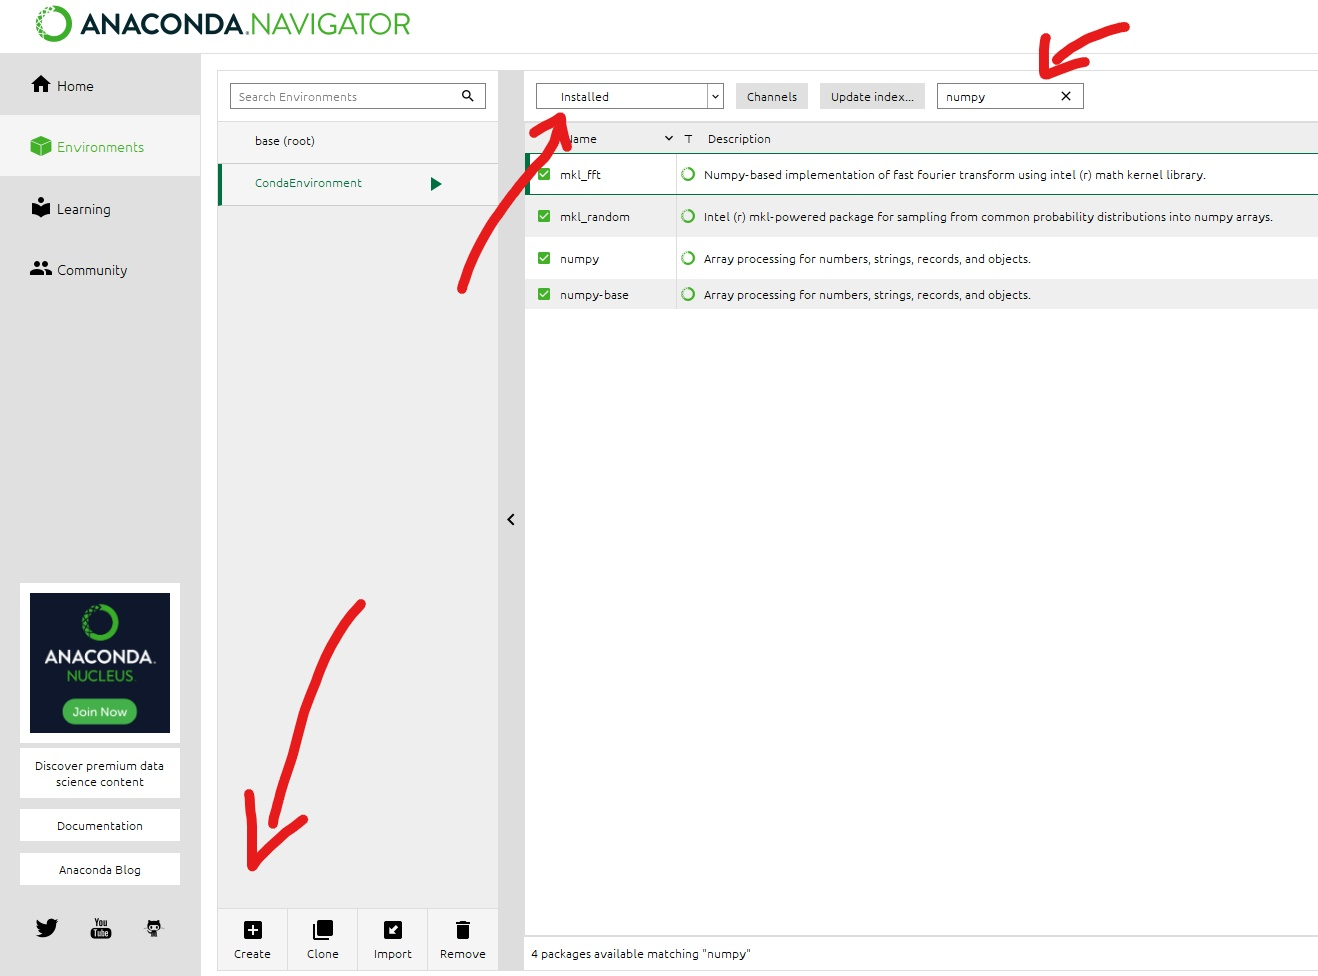
\includegraphics[scale= 0.1]{image/AncaondaEnvironmet.jpg}
        \caption{Anaconda Environments}
        \label{fig:my_label}
    \end{figure}
    \item dall'Ide poi configurare come interprete Conda ed il nome dell'environment che si è creato
     \begin{figure}[h!]
        \centering
        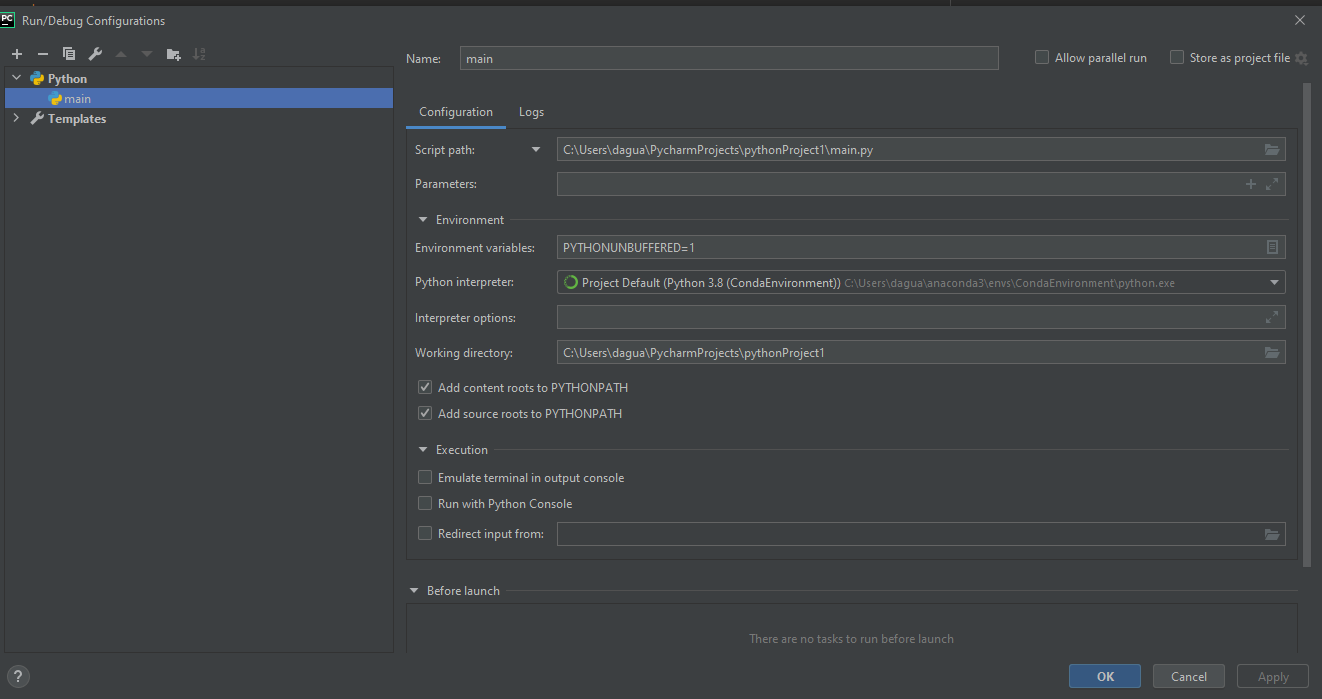
\includegraphics[scale= 0.2]{image/ideEnviroment}
        \caption{IDE Environments}
        \label{fig:my_label}
    \end{figure}
    \item Per \textbf{run} si va su edit configuration icon\textbf{ +} poi \textbf{python} selezionare Conda da \textbf{Python interpreter} dargli un nome e fare attenzione che "Environment variables" sia settata altrimenti creare un nuovo progetto facendo attenzione in fase di creazione di impostare correttamente l'interprete \textbf{Conda}
    \\In "Script Path" trovare inserire la path dello script che bisogna interpretare
     \begin{figure}[h!]
        \centering
        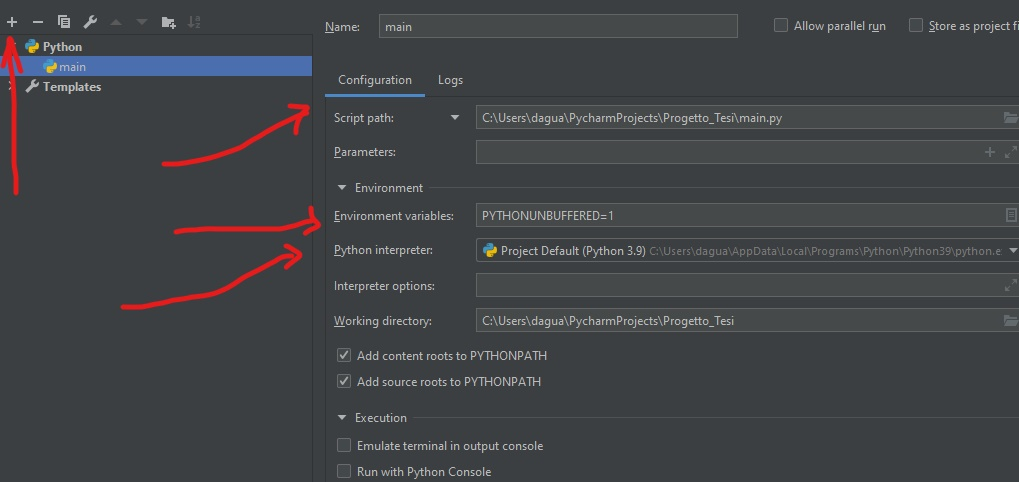
\includegraphics[scale= 0.2]{image/Screenshot (29)_LI.jpg}
        \caption{Porject Environments}
        \label{fig:my_label}
    \end{figure}
\end{enumerate}
\subsection{CSV Library}
INFO: \url{https://docs.python.org/3/library/csv.html}
\\La libreira \textbf{CSV} implementa classi per leggere e scrivere dati tabulari in formato CSV. Consente ai programmatori di dire "scrivere questi dati nel formato preferito da Excel" o "leggere i dati da questo file che è stato generato da Excel", senza conoscere i dettagli precisi del formato CSV utilizzato da Excel. I programmatori possono anche descrivere i formati CSV compresi da altre applicazioni o definire i propri formati CSV speciali.
\subsection{Librosa}
Per installare la libreria in Anaconda \url{https://anaconda.org/conda-forge/librosa}
\\Info: \url{https://librosa.org/doc/latest/index.html}
\\Libreria per leggere e manipolare un file audio

\subsection{Matplotlib}
Importiamo matplotlib per visualizzare l'ampiezza di un suono
\begin{figure}[h!]
        \centering
        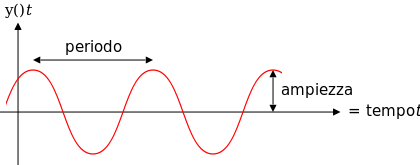
\includegraphics[scale= 0.2]{image/420px-Oscillazione_periodica.svg.png}
        \caption{Ampliezza di un suono}
        \label{fig:my_label}
    \end{figure}

\subsection{Numpy}
Importiamo numpy per la computazione numerica 
\subsection{Os}
INFO: \url{https://docs.python.org/3/library/os.html}
Questo modulo fornisce un modo per utilizzare la funzionalità dipendente dal sistema operativo. Se vuoi solo leggere o scrivere un file vedi \textbf{open()}, se vuoi manipolare i percorsi, vedi il \textbf{os.pathmodulo} e se vuoi leggere tutte le righe in tutti i file sulla linea di comando vedi il\textbf{fileinput} modulo. Per creare file e directory temporanei vedere il \textbf{tempfile} modulo, e per la gestione di file e directory di alto livello vedere il \textbf{shutil} modulo.
\begin{itemize}
    \item \href{ https://www.geeksforgeeks.org/python-os-path-join-method/}{os.path.join - concatena le path}
\end{itemize}
\section{Apk - Andorid App}
App tester sviluppate in API 29
L'apk va inserito in apk > trusted 

\section{Scripts - How Work}
\begin{enumerate}
   \item creare le cartelle nella cartella dove sono gli script 
    \begin{itemize}
        \item Script / apk / audio / trusted
        \\in questa cartella si andrà a generare il file .wav
        \item Script / apk / audio / malware
        \item Script / apk / malware 
        \item Script / trusted 
        \\in questa cartella inseriamo l'applicazione \textbf{.apk}
    \end{itemize}
    \item eseguire lo script test.py
    \\genererà il file .wav 
    \item eseguire lo script progetto2.py
    \\genereraà il file .csv
    \begin{figure}[h]
    \begin{subfigure}{0.5\textwidth}
    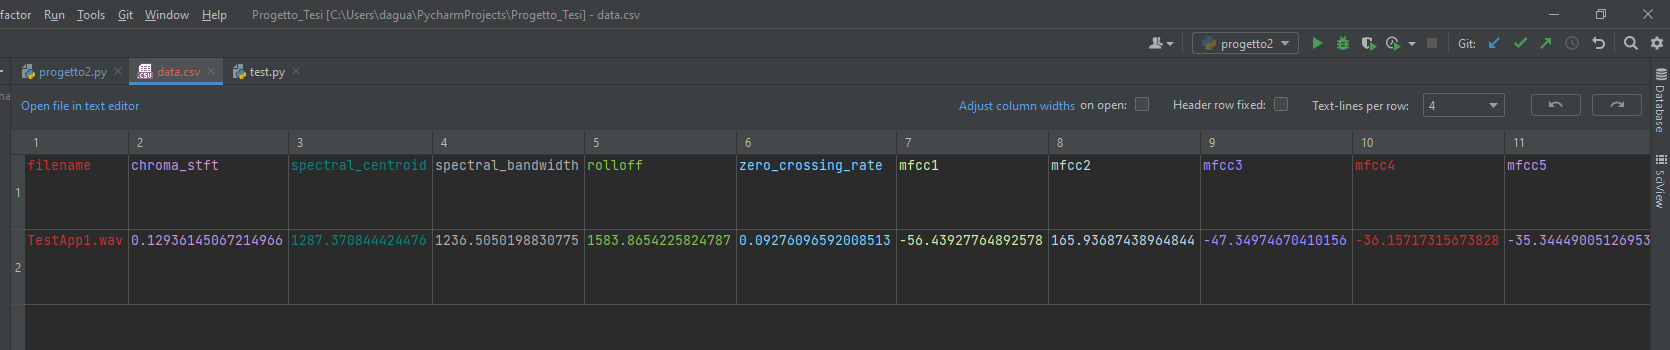
\includegraphics[width=0.9\linewidth, height=5cm]{image/Screenshot (34).png} 
    \caption{data.csv}
    \label{fig:subim1}
    \end{subfigure}
    \begin{subfigure}{0.5\textwidth}
    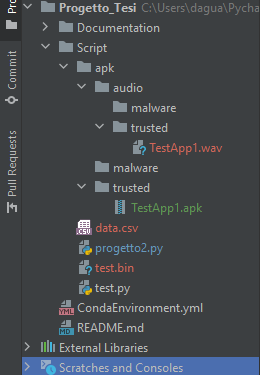
\includegraphics[width=0.9\linewidth, height=5cm]{image/Screenshot (33).png}
    \caption{wav generate}
    \label{fig:subim2}
    \end{subfigure}
    \caption{Subdirectory after scripts}
    \label{fig:image2}
    \end{figure}
\end{enumerate}
\end{document}
